\documentclass[runningheads]{llncs}

\usepackage[T1]{fontenc}
\usepackage{graphicx}
\usepackage{listings}
\usepackage{xcolor}
\usepackage{pdfpages}
\usepackage{hyperref}
\usepackage{url}

\lstset{
    language=HTML,
    basicstyle=\ttfamily\small,
    keywordstyle=\color{blue},
    stringstyle=\color{orange},
    commentstyle=\color{gray},
    breaklines=true,
    frame=single,
    numbers=left,
    numberstyle=\tiny\color{gray},
    showstringspaces=false,
}

\begin{document}

\title{Módulo 1: Los t-warriors}

\author{Manuel Roby Culasso \and
Juan Cruz Solchaga \and
Matteo Pratellesi\and
Mateo Hidalgo\and
Juan Martin Funes Castro}
%

\institute{Universidad Nacional de Cuyo\\
\email{mpratellesidiaz@gmail.com}}
\maketitle

\begin{abstract}
En este trabajo se presentarán los conocimientos adquiridos en el Módulo 1, centrados en el uso de herramientas digitales fundamentales para la formación académica en ingeniería. Se abordan conceptos básicos de Markdown, HTML, LaTeX y notebook, destacando su aplicación en la documentación y estructuración de información.
\end{abstract}

\section{Introducción}

Durante este módulo se trabajó con distintas herramientas orientadas a mejorar la organización y presentación de información técnica. Se desarrollaron ejercicios prácticos que permitieron familiarizarse con lenguajes de marcado y entornos de trabajo utilizados en el ámbito académico y profesional.

El objetivo del informe es mostrar la aplicación de estas herramientas a través de ejemplos concretos, evidenciando su utilidad en la documentación y desarrollo de proyectos.

\section{Archivo README.md}

\subsection{Ejemplo}
\begin{lstlisting}[caption=Ejemplo de README.md]
# Proyecto

## Descripcion
Este proyecto contiene ejercicios del modulo 1.

## Contenido
- HTML
- LaTeX
- Notebooks

[Repositorio](https://github.com)
\end{lstlisting}

\subsection{Descripción}

Se creó y modificó un archivo README.md utilizando sintaxis Markdown, incorporando títulos, listas y enlaces.

\section{Archivo HTML}

\subsection{Ejemplo}
\begin{lstlisting}[language=HTML, caption=Ejemplo HTML]
<!DOCTYPE html>
<html>
<head>
    <title>Pagina</title>
</head>
<body>

<h1>Hola mundo</h1>
<p>Primer pagina HTML</p>

<ul>
<li>Item 1</li>
<li>Item 2</li>
</ul>

</body>
</html>
\end{lstlisting}

\subsection{Descripción}

Se desarrolló un archivo HTML de forma manual, comprendiendo la estructura básica de una página web.

\section{Documento en LaTeX}

\subsection{Ejemplo}
\begin{lstlisting}[language=TeX, caption=Ejemplo LaTeX]
\section{Seccion}
Texto de ejemplo.

\begin{itemize}
\item Punto 1
\item Punto 2
\end{itemize}
\end{lstlisting}

\subsection{Descripción}

Se creó un documento en LaTeX utilizando Overleaf, incorporando secciones y formato estructurado.

\section{Notebooks}

\subsection{Ejemplo}
\begin{lstlisting}[caption=Ejemplo Notebook]
print("Hola mundo")
\end{lstlisting}

\subsection{Descripción}

Se trabajó con notebooks, permitiendo integrar código y texto en un mismo entorno.

\section{Guías de Referencia (Cheatsheets)}

Para la correcta implementación de los lenguajes de marcado y el uso de las herramientas del módulo, se consultaron las siguientes guías rápidas y documentación oficial:

\begin{itemize}
    \item \textbf{Markdown:} \href{https://www.markdownguide.org/cheat-sheet/}{Markdown Guide Cheat Sheet} \cite{markdown}
    \item \textbf{HTML5:} \href{https://www.w3schools.com/tags/default.asp}{W3Schools HTML Reference} \cite{html}
    \item \textbf{LaTeX:} \href{https://www.overleaf.com/learn}{Overleaf Documentation and Wiki} \cite{latex}
    \item \textbf{Git \& GitHub:} \href{https://education.github.com/git-cheat-sheet-education.pdf}{GitHub Education Git Cheat Sheet} \cite{git}
    \item \textbf{Notebooks (Jupyter):} \href{https://jupyter.org/documentation}{Jupyter Documentation} \cite{notebooks}
\end{itemize}


\section{Conclusión}

Este primer módulo me brindó herramientas que transforman significativamente la forma de encarar proyectos técnicos. El mayor aprendizaje radica en comprender la separación entre contenido y formato: a diferencia de los procesadores de texto convencionales, entornos como LaTeX o HTML nos exigen priorizar la estructura lógica de la información antes que su diseño visual.

Asimismo, la utilización de notebooks resulta un gran acierto, ya que unifican el cálculo, el análisis y la documentación en un solo espacio, optimizando la eficiencia. En paralelo, la introducción a GitHub y la creación de archivos README.md me proporcionaron las bases necesarias para estructurar trabajos de forma organizada y fácilmente replicable.

A nivel personal, estoy convencido de que estas metodologías serán fundamentales durante el resto de la carrera, facilitando desde la redacción de informes hasta el desarrollo de proyectos más robustos. A su vez, representan competencias directamente trasladables al ejercicio profesional de la ingeniería, donde la trazabilidad, el orden y la claridad de la información son requisitos indispensables.

\section{Anexos}

\subsection{Currículum}
A continuación, se adjunta el currículum demostrando la aplicación práctica de los estilos de edición aprendidos.

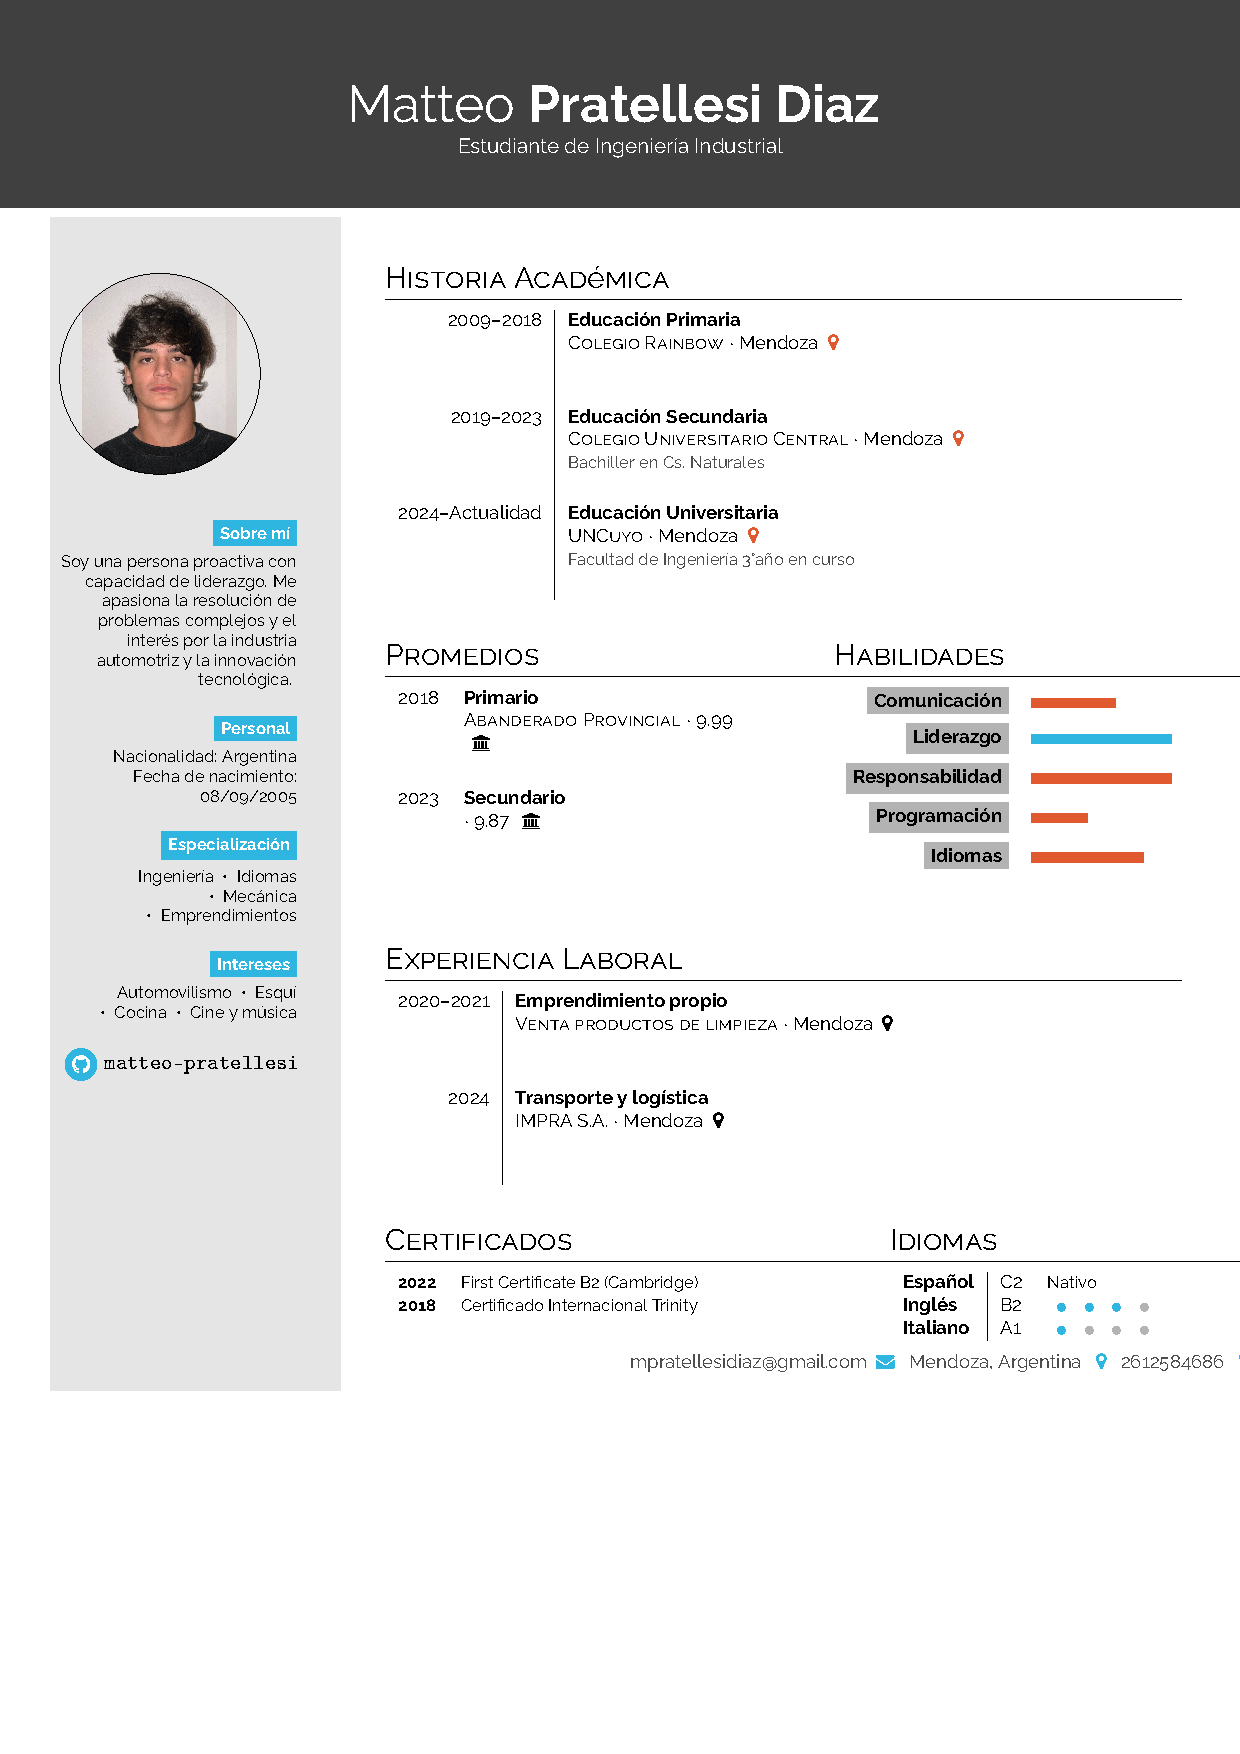
\includepdf[pages=-, pagecommand={\thispagestyle{plain}}]{Matteo Pratellesi CV.pdf}

\bibliographystyle{splncs04}
\bibliography{bibliografia}

\end{document}